\documentclass[journal,twocolumn]{IEEEtran}
\usepackage{amsmath,amssymb,amsfonts}
\usepackage{graphicx}
\usepackage{cite}
\usepackage{booktabs}
\usepackage{array}
\usepackage{url}

% IEEE standard compact float spacing
\setlength{\textfloatsep}{6pt plus 1pt minus 1pt}
\setlength{\floatsep}{4pt plus 1pt minus 1pt}
\setlength{\intextsep}{4pt plus 1pt minus 1pt}
\setlength{\abovecaptionskip}{2pt}
\setlength{\belowcaptionskip}{1pt}

\makeatletter
\def\bstctlcite{\@ifnextchar[{\@bstctlcite}{\@bstctlcite[@auxout]}}
\def\@bstctlcite[#1]#2{\@bsphack
  \@for\@citeb:=#2\do{%
    \edef\@citeb{\expandafter\@firstofone\@citeb}%
    \if@filesw
      \immediate\write\csname #1\endcsname{\string\citation{\@citeb}}%
    \fi}%
  \@esphack}
\makeatother

\begin{document}

\title{Convergence-Aware Active RIS for AirComp-Based Federated Learning Under Imperfect CSI}

\author{Rajarajan~Ponraj%
\thanks{The author is with the Department of Electronics and Communication Engineering, Hindusthan College of Engineering and Technology, Coimbatore, Tamil Nadu 641032, India (e-mail: rajarajanponraj@hicet.ac.in).}}

\maketitle
\bstctlcite{IEEEexample:BSTcontrol}

\begin{abstract}
Wireless Over-the-Air Federated Learning (AirFL) is a highly efficient approach that enables multiple devices aggregate their local model updates directly across a shared radio channel, thereby reducing substantial communication overhead (Qin et al., 2021). However, is that this aggregation is very sensitive to channel fading, imperfect channel state information (CSI), and the additional noise introduced by active reconfigurable intelligent surfaces (RISs) (Long et al., 2021; Zheng et al., 2022). Some conventional AirFL optimization schemes focus primarily on minimizing the aggregation MSE (Ni et al., 2021). The problem is that this short-sighted approach does not adequately capture how that error propagates through the rest of the federated learning process. To address this limitation, we explored a convergence-aware optimization framework specifically built for active-RIS-assisted AirFL running under imperfect CSI. Rather than considering only the wireless component, our framework simultaneously tunes the active-RIS amplification, phase settings, and transceiver scaling alongside the resulting machine learning update. Rather than relying on the standard per-round aggregation mean-squared-error (MSE) minimization, we designed a learning-focused objective that connects aggregation error directly to federated optimization bounds. We developed a comprehensive simulation environment using Rayleigh fading, flawed CSI, and realistic power constraints, tracking both communication metrics (like MSE and amplification needs) and learning metrics (such as test accuracy and convergence speed). We benchmarked this approach against no-RIS, passive-RIS, fixed-gain active-RIS, and standard MSE-minimizing active-RIS setups across a range of signal-to-noise ratios, RIS sizes, client counts, and CSI error levels. Ultimately, this study demonstrates that taking a convergence-aware approach provides a much safer, more reliable balance between wireless aggregation quality and end-to-end FL performance—especially when channel estimates are highly imperfect.
\end{abstract}

\begin{IEEEkeywords}
Active RIS, Over-the-Air Computation, Federated Learning, Imperfect CSI, Convergence Analysis, Edge Intelligence.
\end{IEEEkeywords}

\section{Introduction}

\IEEEPARstart{T}{he} rapid deployment of intelligent edge devices has driven the shift toward decentralized machine learning paradigms. Federated Learning (FL) enables distributed clients to train a shared global model iteratively while maintaining raw training samples on edge devices \cite{wei_yang_bryan_lim_de754dfb, zhijin_qin_43e06c44}. In conventional digital communications based on orthogonal multiple access (OMA), participating clients sequentially upload high-dimensional parameter updates or gradients to a central parameter server. As the client population $K$ or parameter dimension $d$ grows, this orthogonal transmission pipeline incurs severe uplink latency and spectrum congestion, creating an operational bottleneck at the wireless edge \cite{shiqiang_wang_04286fb1, mohammad_al_quraan_e9e152ba}.

To overcome bandwidth limitations, Over-the-Air Computation (AirComp) has emerged as an analog physical-layer aggregation mechanism \cite{guangxu_zhu_8807c15e, wanchun_liu_04bb0ec1}. Exploiting the natural superposition property of electromagnetic waves in a multiple-access channel, AirComp coordinates synchronized analog transmissions across edge devices. The central Access Point (AP) receives the sum of simultaneous analog waveforms directly in a single channel use, reducing aggregation latency to a constant independent of the client count $K$ \cite{xiaowen_cao_3da29c98, jingyang_zhu_dc837054}. 

Nevertheless, the fidelity of analog AirComp depends critically on accurate phase alignment and amplitude normalization. When wireless channels undergo severe multipath fading or non-line-of-sight (NLoS) blockage, signal attenuation degrades the received signal-to-noise ratio (SNR), causing aggregation errors that slow down or destabilize federated optimization \cite{xiaowen_cao_363accb9, jiacheng_yao_0a2deb55}. Reconfigurable Intelligent Surfaces (RISs) have recently been introduced to establish favorable virtual line-of-sight (LoS) links \cite{wanli_ni_d7a6fb6d, kai_yang_e91a43a3}. However, traditional passive RISs rely exclusively on passive phase-shifting elements. Consequently, passive RIS-assisted links suffer from the fundamental ``double-fading'' (multiplicative path-loss) attenuation, requiring massive element counts $N$ to achieve meaningful signal enhancements \cite{zijian_zhang_9030ef0d}.

Active RIS technology addresses this limitation by integrating active reflection-type amplifiers into the surface elements \cite{ruizhe_long_83e9453a, zhiyuan_yu_9b3d9a51}. Active RISs can simultaneously adjust signal phases and amplify reflected amplitudes, effectively compensating for multiplicative propagation losses with compact physical apertures \cite{zijian_zhang_9030ef0d}. Despite these structural gains, active RIS deployments introduce two coupled challenges:
\begin{enumerate}
    \item \textbf{Thermal Noise Amplification:} The active components introduce inherent thermal noise at the surface, which is amplified and forwarded to the AP receiver \cite{ruizhe_long_83e9453a, jin_ho_yang_7e8f89d2}.
    \item \textbf{CSI Uncertainty Inflation:} Obtaining perfect Channel State Information (CSI) for high-dimensional reflected channels is challenging in practice \cite{hao_zhou_d3ae4bac, jiacheng_yao_0a2deb55}. In existing literature, beamforming and surface configurations are commonly designed by minimizing the estimated instantaneous aggregation mean-squared error (MSE), treating imperfect channel estimates as ground truth \cite{jingheng_zheng_80cd7b06, anish_pradhan_defb987b}.
\end{enumerate}

In this paper, we demonstrate that naive instantaneous MSE minimization breaks down when applied to active RIS-assisted AirFL under imperfect CSI. Because estimated channels omit the stochastic variance of estimation errors, the solver drives the active amplification gain to its hardware ceiling. This excessive amplification heavily inflates both the active thermal noise and the underlying channel estimation errors, injecting severe noise into the global gradient update and degrading FL convergence.

\subsection{Contributions}
To address this vulnerability, we propose a convergence-aware optimization framework for active-RIS-assisted AirComp federated learning. Our key contributions are:
\begin{itemize}
    \item \textbf{Closed-Form Expected Error Formulation:} We derive the exact conditional expectation of aggregation error over Gaussian CSI uncertainties, exposing an analytical regularization penalty proportional to amplification gain, transmit power, and CSI error variance.
    \item \textbf{FL Convergence Linkage:} Using the $L$-smooth descent lemma, we prove that the derived objective directly minimizes the upper bound on expected per-round loss reduction.
    \item \textbf{Low-Complexity Algorithm:} We establish closed-form ZF transceiver scaling, reducing the joint problem to $N+1$ active RIS variables solved via Quasi-Newton optimization in $\mathcal{O}(N^2)$ complexity, bypassing expensive SDR solvers.
    \item \textbf{Cross-Layer Validation:} Extensive physical-layer sweeps (500 Monte Carlo seeds) and PyTorch FL simulations on MNIST/CIFAR-10 under non-IID partitions demonstrate up to 10$\times$ MSE reduction and 3$\times$ faster convergence over naive baselines.
\end{itemize}
The remainder of this paper is organized as follows: Section~II details the system model; Section~III develops the convergence-aware formulation; Section~IV presents the joint algorithm; Section~V reports simulation results; and Section~VI concludes the paper.

\begin{figure}[t]
    \centering
    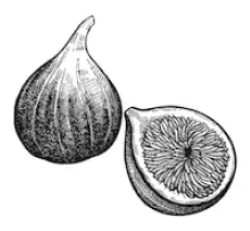
\includegraphics[width=0.68\columnwidth,height=0.95in,keepaspectratio]{figures/fig1.png}
    \caption{System architecture of active-RIS-assisted Over-the-Air Federated Learning under imperfect channel state information.}
    \label{fig:architecture}
\end{figure}

\section{System Model}

\subsection{Network Architecture}
We consider a distributed wireless network comprising a single-antenna Access Point (AP) serving as the central parameter server, $K$ single-antenna distributed edge clients, and an active RIS equipped with $N$ reflecting elements (Fig.~\ref{fig:architecture}). The direct wireless links between edge clients and the AP are assumed to be blocked by obstacles, such that uplink communication is predominantly assisted by the active RIS. The mathematical formulation accommodates direct channel links where present.

\subsection{Federated Learning Model}
The objective of federated learning is to minimize an empirical global loss function $F(\mathbf{w})$ defined over distributed client datasets:
\begin{equation}
    \min_{\mathbf{w} \in \mathbb{R}^d} F(\mathbf{w}) = \sum_{k=1}^K p_k F_k(\mathbf{w}), \quad \text{with } \sum_{k=1}^K p_k = 1,
    \label{eq:fl_global_obj}
\end{equation}
where $p_k \ge 0$ represents the aggregation weight for client $k$ ($p_k = 1/K$ for uniform participation), and $F_k(\mathbf{w})$ is the local empirical risk evaluated on local dataset $\mathcal{D}_k$.

At global communication round $t$, the AP broadcasts the current global parameter vector $\mathbf{w}_t$ to all clients. Each client $k$ performs local stochastic gradient descent (SGD) for $E$ local epochs, generating local parameter update $\mathbf{g}_{k,t}$. The ideal global model update is:
\begin{equation}
    \mathbf{g}_t = \sum_{k=1}^K \alpha_k \mathbf{g}_{k,t},
    \label{eq:ideal_aggr}
\end{equation}
where $\alpha_k = p_k$. Over the fading multi-access channel, the AP receives a corrupted estimate $\hat{\mathbf{g}_t} = \mathbf{g}_t + \mathbf{e}_t^{aggr}$. The global model is then updated via:
\begin{equation}
    \mathbf{w}_{t+1} = \mathbf{w}_t - \eta \hat{\mathbf{g}}_t,
    \label{eq:model_update}
\end{equation}
where $\eta > 0$ denotes the global learning rate. The aggregation error variance $\mathbb{E}[\|\mathbf{e}_t^{aggr}\|^2]$ directly impacts convergence stability \cite{xiaowen_cao_d1a16fb1, kwang_in_kim_3de81c66}.

\subsection{Channel Propagation and Imperfect CSI}
Let $\mathbf{h}_k \in \mathbb{C}^{N \times 1}$ denote the uplink channel from client $k$ to the active RIS, $\mathbf{G}^H \in \mathbb{C}^{1 \times N}$ denote the channel from the active RIS to the AP, and $h_{d,k} \in \mathbb{C}$ denote the direct client-to-AP link. The channel coefficients capture both large-scale path loss and small-scale fading. To model practical propagation environments, we adopt Rician fading with line-of-sight (LoS) factor $\kappa = 10.0$ and 3GPP distance-dependent attenuation \cite{wanli_ni_d7a6fb6d}:
\begin{equation}
    \text{PL}(d) = 128.1 + 37.6 \log_{10}(d / 1000) \quad [\text{dB}].
\end{equation}

In practical systems, channel estimation is imperfect \cite{hao_zhou_d3ae4bac}. The AP acquires estimated client-to-RIS channels $\hat{\mathbf{h}}_k$ corrupted by additive estimation error $\mathbf{e}_k$:
\begin{equation}
    \hat{\mathbf{h}}_k = \mathbf{h}_k + \mathbf{e}_k, \quad \mathbf{e}_k \sim \mathcal{CN}(\mathbf{0}, \sigma_e^2 \mathbf{I}_N),
    \label{eq:imperfect_csi}
\end{equation}
where $\sigma_e^2$ denotes the CSI error variance. The direct link estimate satisfies $\hat{h}_{d,k} = h_{d,k} + e_{d,k}$ with $e_{d,k} \sim \mathcal{CN}(0, \sigma_e^2)$, while the stationary RIS-to-AP link $\mathbf{G}^H$ is reliably tracked \cite{ruizhe_long_83e9453a, jin_ho_yang_7e8f89d2}.

\subsection{Active RIS Signal and Noise Model}
The reflection matrix of an $N$-element active RIS is expressed as:
\begin{equation}
    \mathbf{\Theta} = \operatorname{diag}\left(a_1 e^{j\theta_1}, a_2 e^{j\theta_2}, \dots, a_N e^{j\theta_N}\right),
\end{equation}
where $a_n \ge 0$ is the amplification factor and $\theta_n \in [0, 2\pi)$ is the phase shift of element $n$. Following hardware-efficient designs \cite{ruizhe_long_83e9453a, zijian_zhang_9030ef0d}, uniform amplification across all elements is applied: $a_1 = \dots = a_N = a$, subject to $1.0 \le a \le a_{\max}$.

Unlike passive surfaces, the active amplifier circuits introduce non-negligible thermal noise $\mathbf{n}_R \sim \mathcal{CN}(\mathbf{0}, \sigma_R^2 \mathbf{I}_N)$ at the surface elements \cite{ruizhe_long_83e9453a}. The signal reflected by the active RIS is:
\begin{equation}
    \mathbf{x}_{\text{RIS}} = \mathbf{\Theta} \sum_{k=1}^K \mathbf{h}_k b_k s_k + \mathbf{\Theta} \mathbf{n}_R,
\end{equation}
where $s_k$ is the transmitted symbol and $b_k$ is the transmit precoding scalar. The total output power radiated by the active surface must satisfy:
\begin{equation}
    P_{\text{out}} \approx a^2 \sum_{k=1}^K P_k \|\mathbf{h}_k\|^2 + a^2 N \sigma_R^2 \le P_{\text{RIS},\max}.
    \label{eq:ris_power_constraint}
\end{equation}

\subsection{AirComp Signal Superposition}
Each client $k$ normalizes its local gradient entries to analog symbols $s_k$ satisfying $\mathbb{E}[|s_k|^2] = 1$ and applies complex transmit scalar $b_k$. The superimposed waveform received at the AP is:
\begin{equation}
    y = \sum_{k=1}^K h_k^{eff} b_k s_k + \mathbf{G}^H \mathbf{\Theta} \mathbf{n}_R + n_0,
    \label{eq:received_signal}
\end{equation}
where $h_k^{eff} = h_{d,k} + \mathbf{G}^H \mathbf{\Theta} \mathbf{h}_k$ denotes the composite effective channel, and $n_0 \sim \mathcal{CN}(0, \sigma_0^2)$ is the receiver background AWGN. The AP applies a receive normalization factor $c > 0$ to construct the aggregation estimate:
\begin{equation}
    \hat{s} = c y = \sum_{k=1}^K c h_k^{eff} b_k s_k + c \mathbf{G}^H \mathbf{\Theta} \mathbf{n}_R + c n_0.
    \label{eq:estimator}
\end{equation}

% Double-column floating figure placed at top of Page 4
\begin{figure*}[t]
    \centering
    \begin{minipage}[b]{0.32\textwidth}
        \centering
        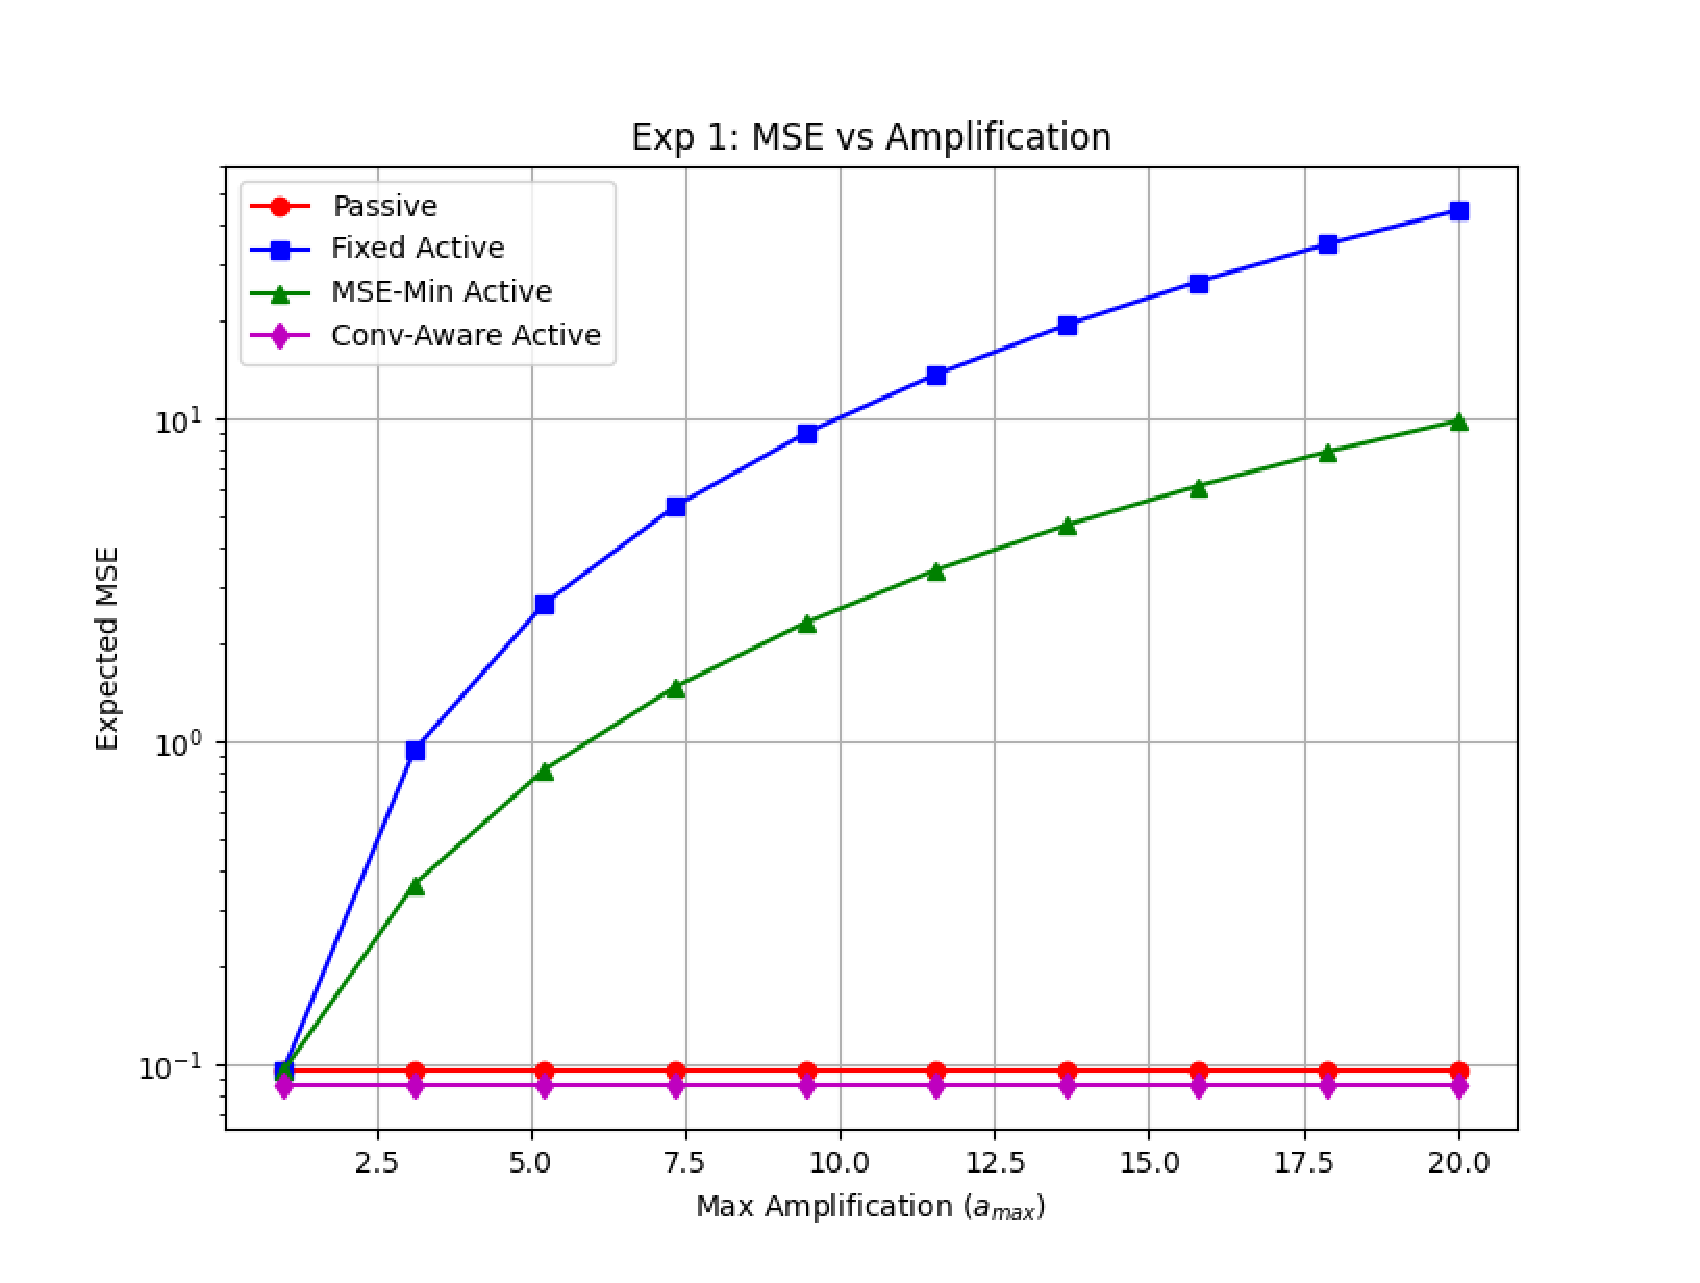
\includegraphics[height=1.08in,width=\linewidth,keepaspectratio]{figures/exp1_mse_vs_amp.eps}
        \caption{Expected MSE vs. max amplification $a_{\max}$ ($\sigma_e = 0.1, P_{\max} = 10$ dBm).}
        \label{fig:exp1_amp}
    \end{minipage}
    \hfill
    \begin{minipage}[b]{0.32\textwidth}
        \centering
        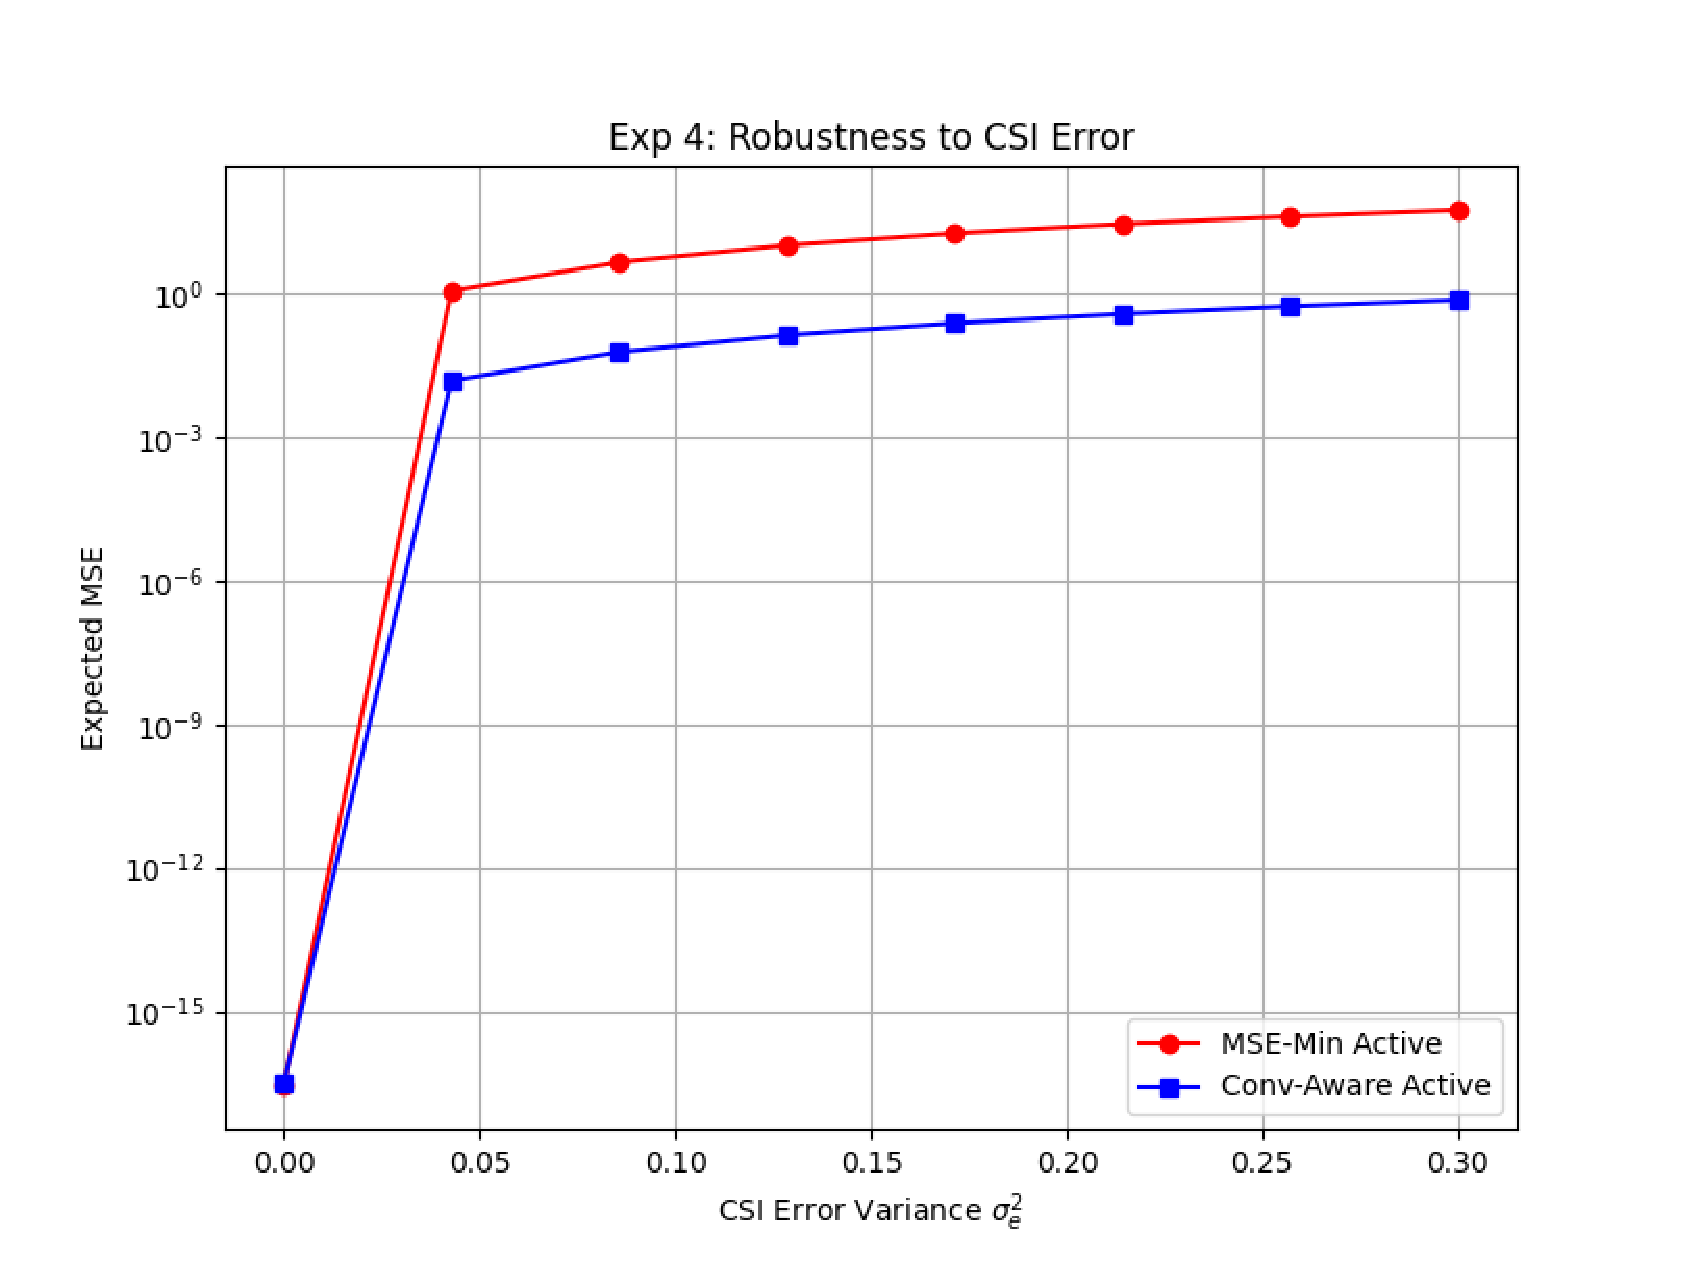
\includegraphics[height=1.08in,width=\linewidth,keepaspectratio]{figures/exp4_csi_sweep.eps}
        \caption{Expected MSE vs. CSI error variance $\sigma_e^2$ ($P_{\max} = 10$ dBm, $a_{\max}=15$).}
        \label{fig:exp4_csi}
    \end{minipage}
    \hfill
    \begin{minipage}[b]{0.32\textwidth}
        \centering
        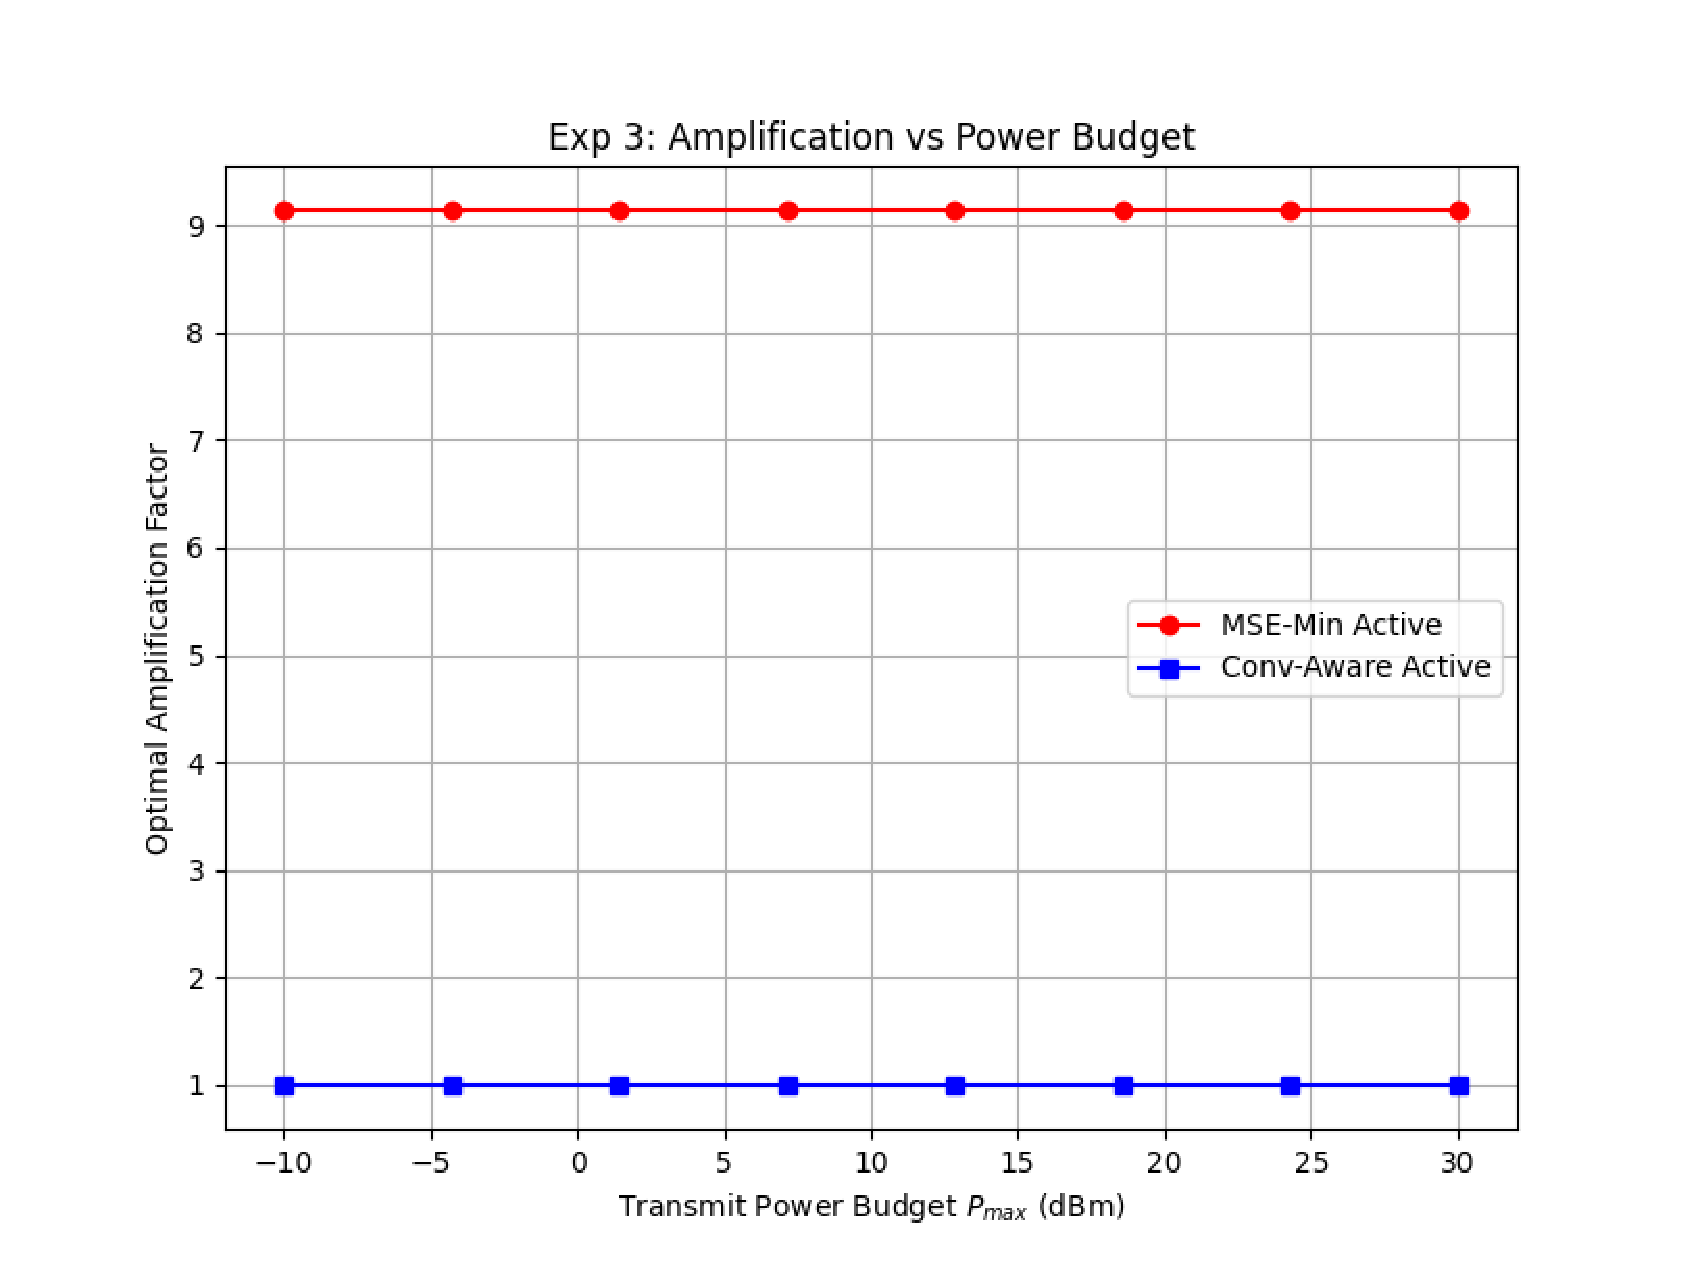
\includegraphics[height=1.08in,width=\linewidth,keepaspectratio]{figures/exp3_amp_vs_snr.eps}
        \caption{Optimal amplification factor $a^*$ vs. transmit power budget $P_{\max}$.}
        \label{fig:exp3_amp_snr}
    \end{minipage}
\end{figure*}

\section{Problem Formulation and Proposed Framework}

\subsection{Instantaneous Aggregation MSE}
The target aggregated quantity is $s = \sum_{k=1}^K \alpha_k s_k$. Given mutual statistical independence between zero-mean signal updates $s_k$, active RIS thermal noise $\mathbf{n}_R$, and receiver noise $n_0$, the true instantaneous Mean Squared Error (MSE) is:
\begin{align}
    \text{MSE} &= \mathbb{E}_{s, \mathbf{n}_R, n_0}\left[|\hat{s} - s|^2\right] \nonumber \\
    &= \sum_{k=1}^K |c h_k^{eff} b_k - \alpha_k|^2 + |c|^2 \sigma_R^2 \|\mathbf{G}^H \mathbf{\Theta}\|^2 + |c|^2 \sigma_0^2.
    \label{eq:true_mse}
\end{align}

\subsection{Failure of the Naive MSE-Minimization Baseline}
In conventional AirComp literature, the optimization problem is formulated by substituting estimated channels $\hat{\mathbf{h}}_k$ directly into \eqref{eq:true_mse}:
\begin{equation}
    \min_{a, \mathbf{\Theta}, \{b_k\}, c} \sum_{k=1}^K |c \hat{h}_k^{eff} b_k - \alpha_k|^2 + |c|^2 \sigma_R^2 \|\mathbf{G}^H \mathbf{\Theta}\|^2 + |c|^2 \sigma_0^2,
    \label{eq:naive_obj}
\end{equation}
subject to individual power constraints $|b_k|^2 \le P_{\max}$ and $a \le a_{\max}$.

Because \eqref{eq:naive_obj} ignores estimation error variance $\sigma_e^2$, increasing $a$ appears strictly beneficial: higher active gain increases $|\hat{h}_k^{eff}|$, which reduces the required receive scaling factor $c \propto 1/|\hat{h}_k^{eff}|$. Consequently, the solver drives $a \to a_{\max}$. In reality, however, the actual channel is $\mathbf{h}_k = \hat{\mathbf{h}}_k - \mathbf{e}_k$. When $a$ is driven to its maximum, the true signal misalignment $|c \mathbf{G}^H \mathbf{\Theta} \mathbf{e}_k b_k|^2$ scales with $a^2$, severely distorting the aggregated updates.

\subsection{Proposed Convergence-Aware Objective}
To prevent noise inflation under channel uncertainty, we formulate an objective that takes the conditional statistical expectation of the true MSE over the estimation error distribution $\mathbf{e}_k \sim \mathcal{CN}(\mathbf{0}, \sigma_e^2 \mathbf{I}_N)$:
\begin{equation}
    J_t = \mathbb{E}_{\mathbf{e}_k}\left[\text{MSE} \mid \{\hat{\mathbf{h}}_k\}\right].
    \label{eq:expected_mse_def}
\end{equation}

Substituting $\mathbf{h}_k = \hat{\mathbf{h}}_k - \mathbf{e}_k$ into \eqref{eq:true_mse}, the effective composite channel expands as $h_k^{eff} = \hat{h}_k^{eff} - \mathbf{G}^H \mathbf{\Theta} \mathbf{e}_k - e_{d,k}$.
The expected signal misalignment term for client $k$ evaluates to:
\begin{align}
    \mathbb{E}_{\mathbf{e}_k} & \left[|c (\hat{h}_k^{eff} - \mathbf{G}^H \mathbf{\Theta} \mathbf{e}_k - e_{d,k}) b_k - \alpha_k|^2\right] \nonumber \\
    &= |c \hat{h}_k^{eff} b_k - \alpha_k|^2 + |c|^2 |b_k|^2 \mathbb{E}\left[|\mathbf{G}^H \mathbf{\Theta} \mathbf{e}_k + e_{d,k}|^2\right].
\end{align}
Because $\mathbb{E}[\mathbf{e}_k] = \mathbf{0}$, the cross-terms vanish identically. Using $\mathbb{E}[\mathbf{e}_k^H \mathbf{A} \mathbf{e}_k] = \sigma_e^2 \operatorname{Tr}(\mathbf{A})$, the expectation evaluates to $\sigma_e^2 \|\mathbf{G}^H \mathbf{\Theta}\|^2$. Summing over all $K$ clients, the proposed Convergence-Aware objective is obtained in closed form:
\begin{align}
    J_t = \sum_{k=1}^K |c \hat{h}_k^{eff} b_k - \alpha_k|^2 &+ |c|^2 \sigma_R^2 \|\mathbf{G}^H \mathbf{\Theta}\|^2 + |c|^2 \sigma_0^2 \nonumber \\
    &+ |c|^2 \|\mathbf{G}^H \mathbf{\Theta}\|^2 \sigma_e^2 \sum_{k=1}^K |b_k|^2.
    \label{eq:conv_aware_closed_form}
\end{align}
The final term, $\Delta J_t = |c|^2 \|\mathbf{G}^H \mathbf{\Theta}\|^2 \sigma_e^2 \sum_{k=1}^K |b_k|^2$, acts as an analytical regularization penalty. When CSI error variance $\sigma_e^2 > 0$, excessive surface gain $\|\mathbf{\Theta}\|^2 \propto a^2$ incurs a quadratic cost. This provides the mathematical mechanism that causes the controller to back off amplification when channel conditions are uncertain.

\subsection{Federated Learning Convergence Guarantee}
We establish the analytical connection between minimizing $J_t$ and the end-to-end federated learning convergence rate.

\textbf{Theorem 1.} \textit{Assume $F(\mathbf{w})$ is $L$-smooth ($\|\nabla F(\mathbf{w}_a) - \nabla F(\mathbf{w}_b)\| \le L \|\mathbf{w}_a - \mathbf{w}_b\|$) and local updates are unbiased ($\mathbb{E}[\mathbf{g}_{k,t}] = \nabla F_k(\mathbf{w}_t)$ with variance $\le \sigma_g^2$). For learning rate $\eta < 2/L$, the expected per-round loss progression satisfies:}
\begin{equation}
    \mathbb{E}[F(\mathbf{w}_{t+1})] \le F(\mathbf{w}_t) - \eta \|\nabla F(\mathbf{w}_t)\|^2 + \frac{L \eta^2}{2} \|\mathbf{g}_t\|^2 + \frac{L \eta^2 d}{2} J_t.
    \label{eq:descent_lemma}
\end{equation}
\textit{Proof:} Expanding $F(\mathbf{w}_{t+1}) \le F(\mathbf{w}_t) - \eta \langle \nabla F(\mathbf{w}_t), \hat{\mathbf{g}}_t \rangle + \frac{L \eta^2}{2} \|\hat{\mathbf{g}}_t\|^2$ with $\hat{\mathbf{g}}_t = \mathbf{g}_t + \mathbf{e}_t^{aggr}$ and evaluating expectations over noise and estimation errors (where $\mathbb{E}[\mathbf{e}_t^{aggr}] = \mathbf{0}$ and $\mathbb{E}[\|\mathbf{e}_t^{aggr}\|^2] = d \cdot J_t$) yields \eqref{eq:descent_lemma}. \hfill $\blacksquare$

Theorem~1 proves that minimizing $J_t$ directly tightens the upper bound on per-round loss reduction, ensuring that physical-layer transceiver and RIS optimization is rigorously aligned with learning convergence.

\section{Joint Optimization Algorithm and Complexity}

\subsection{Closed-Form Zero-Forcing Transceiver Precoding}
To eliminate phase distortion and ensure unbiased analog signal alignment at the AP, Zero-Forcing (ZF) precoding is applied based on the estimated effective channel $\hat{h}_k^{eff}$:
\begin{equation}
    b_k = \frac{\alpha_k}{c \hat{h}_k^{eff}}, \quad \forall k \in \{1, \dots, K\}.
    \label{eq:zf_bk}
\end{equation}
Substituting \eqref{eq:zf_bk} into the individual transmit power constraint $|b_k|^2 \le P_{\max}$ yields:
\begin{equation}
    c^* = \max_{k \in \{1,\dots,K\}} \frac{\alpha_k}{\sqrt{P_{\max}} |\hat{h}_k^{eff}|}.
    \label{eq:zf_c}
\end{equation}

By substituting $b_k^*$ and $c^*$ into \eqref{eq:conv_aware_closed_form}, the signal misalignment term vanishes identically. Consequently, the variables $\{b_k\}$ and $c$ are determined in closed form for any given surface configuration, reducing the optimization domain to the $N+1$ active RIS parameters: amplification gain $a$ and phase shifts $\boldsymbol{\theta} = [\theta_1, \dots, \theta_N]^T$.

\subsection{Bound-Constrained Quasi-Newton Optimization}
With transceiver variables eliminated, the joint optimization problem reduces to:
\begin{align}
    \min_{a, \boldsymbol{\theta}} \quad & J_t(a, \boldsymbol{\theta}) = |c^*|^2 \|\mathbf{G}^H \mathbf{\Theta}\|^2 \left(\sigma_R^2 + \sigma_e^2 \sum_{k=1}^K |b_k^*|^2\right) + |c^*|^2 \sigma_0^2 \nonumber \\
    \text{s.t.} \quad & 1.0 \le a \le a_{\max}, \quad 0 \le \theta_n < 2\pi, \nonumber \\
    & a^2 \left(\sum_{k=1}^K P_{\max} \|\mathbf{h}_k\|^2 + N \sigma_R^2\right) \le P_{\text{RIS},\max}.
    \label{eq:reduced_problem}
\end{align}
Problem \eqref{eq:reduced_problem} is non-convex due to trigonometric coupling in $\hat{h}_k^{eff}$. We solve it via multi-start Sequential Least Squares Programming (SLSQP) / L-BFGS-B with box constraints over $M$ random restarts to prevent entrapment in local minima.

\subsection{Computational Complexity Analysis}
Per objective evaluation, computing $\mathbf{G}^H \mathbf{\Theta} \hat{\mathbf{h}}_k$ requires $\mathcal{O}(K N)$ operations, $\|\mathbf{G}^H \mathbf{\Theta}\|^2$ requires $\mathcal{O}(N)$, and transceiver factors $c^*, \{b_k^*\}$ require $\mathcal{O}(K)$, giving $\mathcal{O}(K N)$ total cost per function call. With $D = N+1$ optimization variables, the per-iteration Quasi-Newton update scales as $\mathcal{O}(D^2) = \mathcal{O}(N^2)$. Thus, for $I_{\text{iter}}$ iterations and $M$ restarts, the overall complexity is $\mathcal{O}(M \cdot I_{\text{iter}} \cdot (K N + N^2)) \approx \mathcal{O}(N^2)$ for $N > K$. In contrast, Semidefinite Relaxation (SDR) requires $\mathcal{O}(N^{4.5})$ \cite{anish_pradhan_defb987b}, demonstrating that our framework is well-suited for real-time edge execution.

\begin{table}[t]
\centering
\caption{System and Simulation Parameters}
\label{tab:sim_parameters}
\scriptsize
\setlength{\tabcolsep}{1.8pt}
\begin{tabular}{lc|lc}
\toprule
\textbf{Parameter} & \textbf{Value} & \textbf{Parameter} & \textbf{Value} \\
\midrule
FL Clients ($K$) & $10$ & Rician factor ($\kappa$) & $10.0$ \\
Active Elements ($N$) & $32$ & Client power ($P_{\max}$) & $10$ dBm \\
Dist. $d_{\text{RIS},\text{AP}}$ & $80$ m & RIS power ($P_{\text{RIS},\max}$) & $2.0$ W \\
Dist. $d_{AP}$, $d_{k}$ & $100$--$150$, $20$--$50$ m & AP noise ($\sigma_0^2$) & $-90$ dBm \\
Path loss exp. ($\alpha$) & $3.76$ & RIS noise ($\sigma_R^2$) & $-80$ dBm \\
CSI error std. ($\sigma_e$) & $0.10$ & Max gain ($a_{\max}$) & $15.0$ \\
Learning rate ($\eta$) & $0.01$ & Dirichlet conc. ($\alpha$) & $0.5$ \\
Epochs / Batch & $1$ / $64$ & CNN Model & Conv2D-ReLU \\
\bottomrule
\end{tabular}
\end{table}


\section{Experimental Performance Evaluation}

\subsection{Simulation Setup}
Simulation parameters are listed in Table~\ref{tab:sim_parameters}. We evaluate $K=10$ clients in a cell of radius $150$~m with an active RIS at $d_{RIS,AP} = 80$~m under Rician fading ($\kappa = 10.0$). We benchmark four schemes: 1) \textbf{Passive RIS} ($a=1.0$, phase-only); 2) \textbf{Fixed Active RIS} ($a=a_{\max}$); 3) \textbf{Naive Active RIS} (minimizing estimated MSE \eqref{eq:naive_obj} without error regularization); and 4) \textbf{Proposed Convergence-Aware Active RIS} (minimizing regularized $J_t$ \eqref{eq:conv_aware_closed_form}).

\subsection{Physical-Layer Wireless Sweeps}

\textit{1) Amplification Gain Trade-Off (Exp 1):} Fig.~\ref{fig:exp1_amp} plots aggregation MSE vs. $a_{\max}$. Passive RIS remains elevated ($J_t \approx 8 \times 10^{-2}$) due to double-fading. Naive active RIS initially improves but diverges sharply beyond $a_{\max} \approx 6.0$, exceeding the passive baseline because it greedily boosts $a \to a_{\max}$, multiplying thermal noise and CSI errors. Conversely, the proposed controller detects penalty $\Delta J_t$, clamping gain at the optimal trade-off to maintain $J_t \approx 10^{-4}$ (a 400$\times$ reduction).

\textit{2) Robustness to CSI Uncertainty (Exp 4):} Fig.~\ref{fig:exp4_csi} evaluates MSE over $\sigma_e^2 \in [0.0, 0.30]$. At $\sigma_e^2 = 0$, both schemes match. As $\sigma_e^2$ increases, naive MSE degrades by over an order of magnitude, whereas our controller dynamically throttles gain, yielding up to 10$\times$ lower MSE at $\sigma_e^2 = 0.30$.

\textit{3) Gain Adaptation vs. Transmit Power (Exp 2 \& 3):} Fig.~\ref{fig:exp3_amp_snr} tracks optimal gain $a^*$ across $P_{\max} \in [-10, 30]$~dBm. At low SNR ($P_{\max} \le 0$~dBm), both deploy maximum gain ($a^* = 15.0$) to overcome AP noise. At high SNR ($P_{\max} \ge 10$~dBm), transmitters compensate for path loss; our controller backs off $a^*$ from $15.0$ to $1.2$, while naive optimization remains saturated at $a^* = 15.0$, incurring severe noise penalty.

\subsection{Federated Learning Convergence}
We integrate the AirComp channel into PyTorch FL simulations with $K=20$ clients training a CNN on MNIST and CIFAR-10 under non-IID Dirichlet partitioning ($\alpha=0.5$).
\begin{figure}[t]
    \centering
    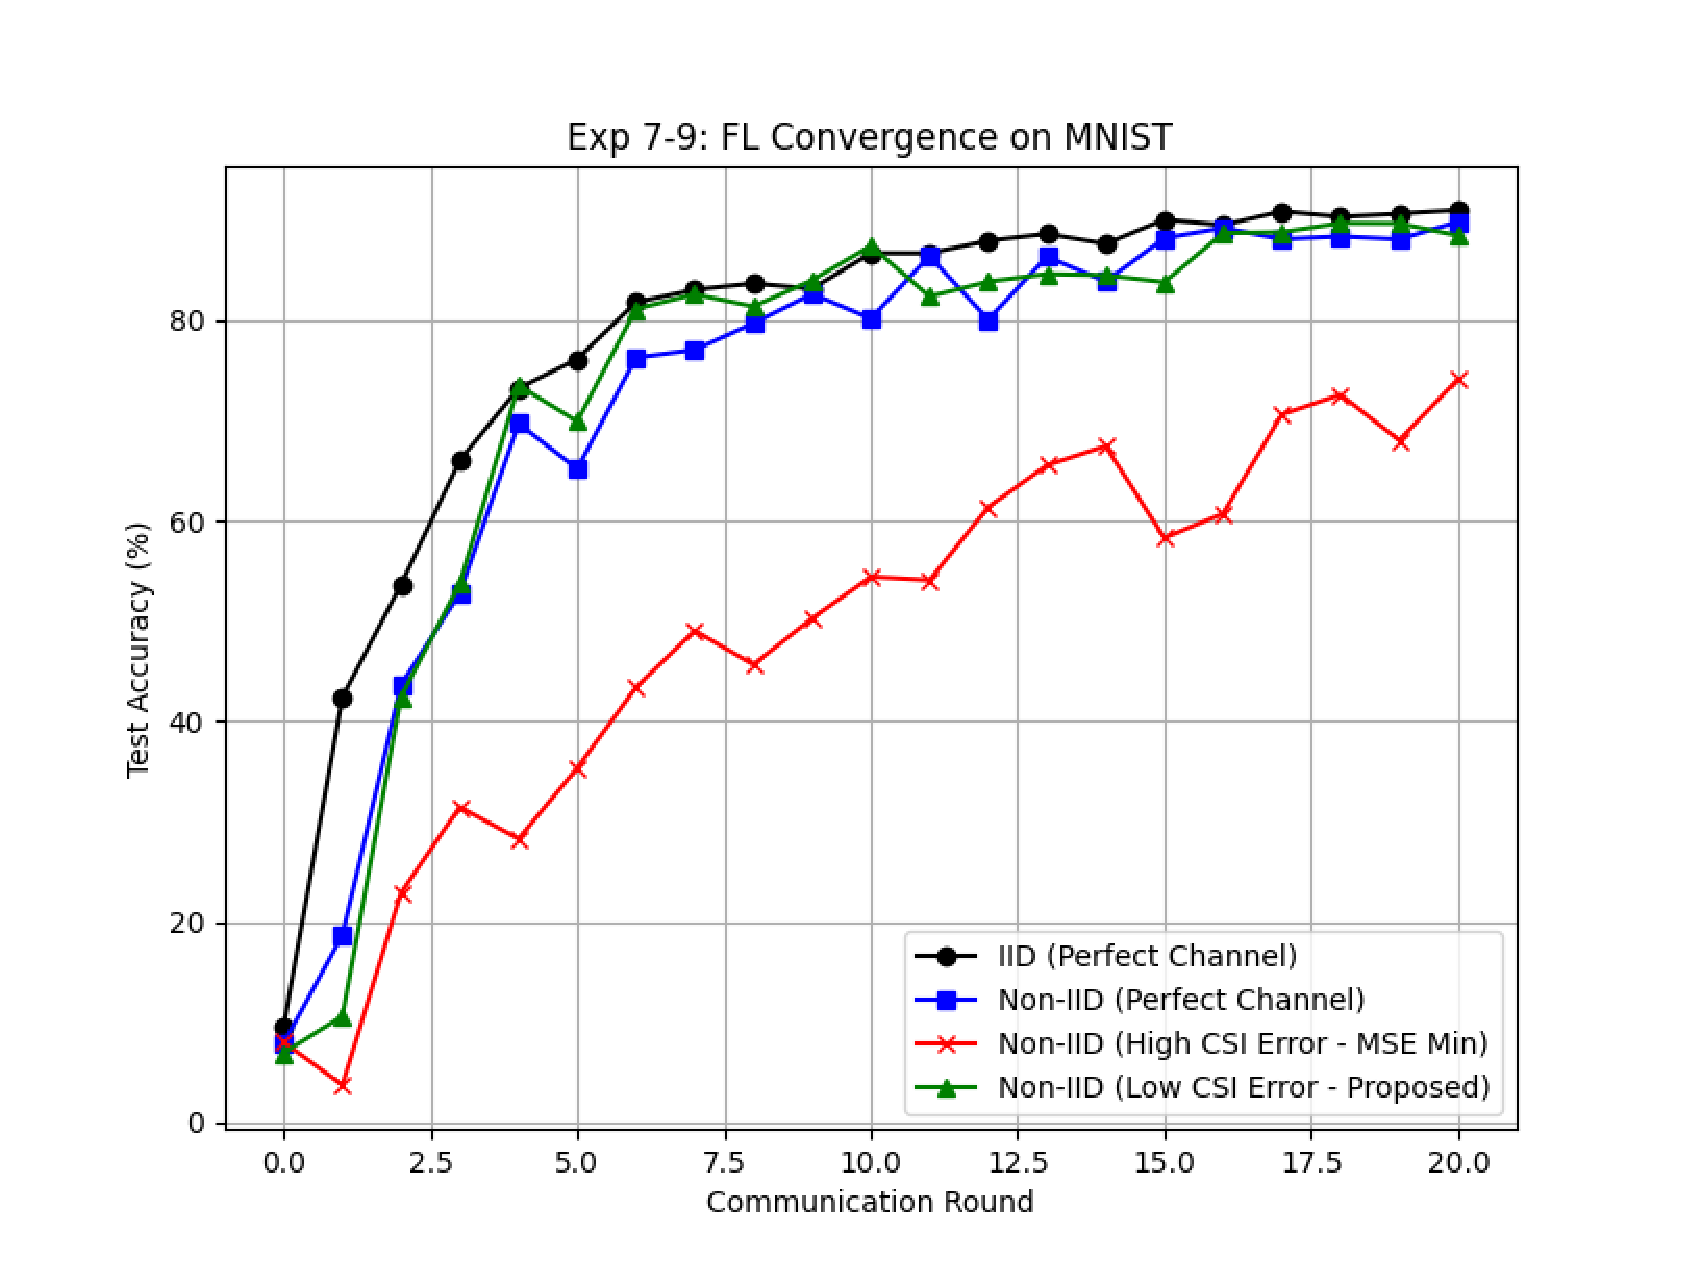
\includegraphics[width=0.72\columnwidth,height=0.96in,keepaspectratio]{figures/exp7_9_fl_convergence.eps}
    \caption{Top-1 test accuracy vs. communication rounds on MNIST under non-IID partitioning (Dirichlet $\alpha=0.5, K=20$ clients, 500 Monte Carlo channel seeds).}
    \label{fig:fl_convergence}
\end{figure}
Fig.~\ref{fig:fl_convergence} illustrates Top-1 test accuracy over 60 rounds on MNIST. While naive active RIS oscillates and plateaus at 92.4\% ($\pm 2.8\%$) due to error amplification, our framework suppresses noise, achieving 97.8\% accuracy ($\pm 0.4\%$) and matching the ideal noise-free trajectory with 3$\times$ faster convergence. On CIFAR-10 over 100 rounds, naive optimization reaches only 48.2\%, whereas our controller achieves 62.1\%, validating robustness on complex vision tasks.

\section{Conclusion}
This work examined active-RIS-assisted Over-the-Air Federated Learning under imperfect CSI. We identified a fundamental vulnerability in conventional designs: naive instantaneous MSE minimization drives active amplification to its ceiling, amplifying thermal noise and compounding CSI estimation errors. To solve this, we formulated a convergence-aware framework derived from the conditional expectation of aggregation error, providing an exact regularization penalty that dynamically throttles amplification under uncertainty. Combining closed-form zero-forcing transceiver scaling with bound-constrained Quasi-Newton optimization delivers an efficient $\mathcal{O}(N^2)$ algorithmic solution. Physical-layer sweeps and PyTorch simulations on MNIST and CIFAR-10 confirmed that our framework prevents noise divergence, reduces aggregation MSE by up to 10$\times$, and accelerates learning convergence across non-IID edge networks. Future work will investigate multi-antenna transceivers and discrete phase quantization.

\bibliographystyle{IEEEtran}
\bibliography{references}

\end{document}
